% Options for packages loaded elsewhere
\PassOptionsToPackage{unicode}{hyperref}
\PassOptionsToPackage{hyphens}{url}
%
\documentclass[
]{article}
\usepackage{amsmath,amssymb}
\usepackage{iftex}
\ifPDFTeX
  \usepackage[T1]{fontenc}
  \usepackage[utf8]{inputenc}
  \usepackage{textcomp} % provide euro and other symbols
\else % if luatex or xetex
  \usepackage{unicode-math} % this also loads fontspec
  \defaultfontfeatures{Scale=MatchLowercase}
  \defaultfontfeatures[\rmfamily]{Ligatures=TeX,Scale=1}
\fi
\usepackage{lmodern}
\ifPDFTeX\else
  % xetex/luatex font selection
\fi
% Use upquote if available, for straight quotes in verbatim environments
\IfFileExists{upquote.sty}{\usepackage{upquote}}{}
\IfFileExists{microtype.sty}{% use microtype if available
  \usepackage[]{microtype}
  \UseMicrotypeSet[protrusion]{basicmath} % disable protrusion for tt fonts
}{}
\makeatletter
\@ifundefined{KOMAClassName}{% if non-KOMA class
  \IfFileExists{parskip.sty}{%
    \usepackage{parskip}
  }{% else
    \setlength{\parindent}{0pt}
    \setlength{\parskip}{6pt plus 2pt minus 1pt}}
}{% if KOMA class
  \KOMAoptions{parskip=half}}
\makeatother
\usepackage{xcolor}
\usepackage[margin=1in]{geometry}
\usepackage{color}
\usepackage{fancyvrb}
\newcommand{\VerbBar}{|}
\newcommand{\VERB}{\Verb[commandchars=\\\{\}]}
\DefineVerbatimEnvironment{Highlighting}{Verbatim}{commandchars=\\\{\}}
% Add ',fontsize=\small' for more characters per line
\usepackage{framed}
\definecolor{shadecolor}{RGB}{248,248,248}
\newenvironment{Shaded}{\begin{snugshade}}{\end{snugshade}}
\newcommand{\AlertTok}[1]{\textcolor[rgb]{0.94,0.16,0.16}{#1}}
\newcommand{\AnnotationTok}[1]{\textcolor[rgb]{0.56,0.35,0.01}{\textbf{\textit{#1}}}}
\newcommand{\AttributeTok}[1]{\textcolor[rgb]{0.13,0.29,0.53}{#1}}
\newcommand{\BaseNTok}[1]{\textcolor[rgb]{0.00,0.00,0.81}{#1}}
\newcommand{\BuiltInTok}[1]{#1}
\newcommand{\CharTok}[1]{\textcolor[rgb]{0.31,0.60,0.02}{#1}}
\newcommand{\CommentTok}[1]{\textcolor[rgb]{0.56,0.35,0.01}{\textit{#1}}}
\newcommand{\CommentVarTok}[1]{\textcolor[rgb]{0.56,0.35,0.01}{\textbf{\textit{#1}}}}
\newcommand{\ConstantTok}[1]{\textcolor[rgb]{0.56,0.35,0.01}{#1}}
\newcommand{\ControlFlowTok}[1]{\textcolor[rgb]{0.13,0.29,0.53}{\textbf{#1}}}
\newcommand{\DataTypeTok}[1]{\textcolor[rgb]{0.13,0.29,0.53}{#1}}
\newcommand{\DecValTok}[1]{\textcolor[rgb]{0.00,0.00,0.81}{#1}}
\newcommand{\DocumentationTok}[1]{\textcolor[rgb]{0.56,0.35,0.01}{\textbf{\textit{#1}}}}
\newcommand{\ErrorTok}[1]{\textcolor[rgb]{0.64,0.00,0.00}{\textbf{#1}}}
\newcommand{\ExtensionTok}[1]{#1}
\newcommand{\FloatTok}[1]{\textcolor[rgb]{0.00,0.00,0.81}{#1}}
\newcommand{\FunctionTok}[1]{\textcolor[rgb]{0.13,0.29,0.53}{\textbf{#1}}}
\newcommand{\ImportTok}[1]{#1}
\newcommand{\InformationTok}[1]{\textcolor[rgb]{0.56,0.35,0.01}{\textbf{\textit{#1}}}}
\newcommand{\KeywordTok}[1]{\textcolor[rgb]{0.13,0.29,0.53}{\textbf{#1}}}
\newcommand{\NormalTok}[1]{#1}
\newcommand{\OperatorTok}[1]{\textcolor[rgb]{0.81,0.36,0.00}{\textbf{#1}}}
\newcommand{\OtherTok}[1]{\textcolor[rgb]{0.56,0.35,0.01}{#1}}
\newcommand{\PreprocessorTok}[1]{\textcolor[rgb]{0.56,0.35,0.01}{\textit{#1}}}
\newcommand{\RegionMarkerTok}[1]{#1}
\newcommand{\SpecialCharTok}[1]{\textcolor[rgb]{0.81,0.36,0.00}{\textbf{#1}}}
\newcommand{\SpecialStringTok}[1]{\textcolor[rgb]{0.31,0.60,0.02}{#1}}
\newcommand{\StringTok}[1]{\textcolor[rgb]{0.31,0.60,0.02}{#1}}
\newcommand{\VariableTok}[1]{\textcolor[rgb]{0.00,0.00,0.00}{#1}}
\newcommand{\VerbatimStringTok}[1]{\textcolor[rgb]{0.31,0.60,0.02}{#1}}
\newcommand{\WarningTok}[1]{\textcolor[rgb]{0.56,0.35,0.01}{\textbf{\textit{#1}}}}
\usepackage{graphicx}
\makeatletter
\def\maxwidth{\ifdim\Gin@nat@width>\linewidth\linewidth\else\Gin@nat@width\fi}
\def\maxheight{\ifdim\Gin@nat@height>\textheight\textheight\else\Gin@nat@height\fi}
\makeatother
% Scale images if necessary, so that they will not overflow the page
% margins by default, and it is still possible to overwrite the defaults
% using explicit options in \includegraphics[width, height, ...]{}
\setkeys{Gin}{width=\maxwidth,height=\maxheight,keepaspectratio}
% Set default figure placement to htbp
\makeatletter
\def\fps@figure{htbp}
\makeatother
\setlength{\emergencystretch}{3em} % prevent overfull lines
\providecommand{\tightlist}{%
  \setlength{\itemsep}{0pt}\setlength{\parskip}{0pt}}
\setcounter{secnumdepth}{-\maxdimen} % remove section numbering
\usepackage{booktabs}
\usepackage{longtable}
\usepackage{array}
\usepackage{multirow}
\usepackage{wrapfig}
\usepackage{float}
\usepackage{colortbl}
\usepackage{pdflscape}
\usepackage{tabu}
\usepackage{threeparttable}
\usepackage{threeparttablex}
\usepackage[normalem]{ulem}
\usepackage{makecell}
\usepackage{xcolor}
\ifLuaTeX
  \usepackage{selnolig}  % disable illegal ligatures
\fi
\IfFileExists{bookmark.sty}{\usepackage{bookmark}}{\usepackage{hyperref}}
\IfFileExists{xurl.sty}{\usepackage{xurl}}{} % add URL line breaks if available
\urlstyle{same}
\hypersetup{
  pdftitle={Homework MBIO 612},
  pdfauthor={Retno K. Ningrum},
  hidelinks,
  pdfcreator={LaTeX via pandoc}}

\title{Homework MBIO 612}
\usepackage{etoolbox}
\makeatletter
\providecommand{\subtitle}[1]{% add subtitle to \maketitle
  \apptocmd{\@title}{\par {\large #1 \par}}{}{}
}
\makeatother
\subtitle{Rmarkdown}
\author{Retno K. Ningrum}
\date{2024-10-08}

\begin{document}
\maketitle

{
\setcounter{tocdepth}{2}
\tableofcontents
}
\hypertarget{direction}{%
\section{Direction}\label{direction}}

Take any data sheets you have already worked with, create at least one
table and one figure in Rmarkdown file. Create in either html, github
doc, or pdf format (you must knit the file). Make sure you have headings
with clear explainations of what you are doing. Practice the bold,
italics, and lists. make sure your outputs and script are saved in the
appropriate folders. keep proper coding etiquette.

\hypertarget{sea-turtle-nesting-sites}{%
\section{Sea Turtle Nesting Sites}\label{sea-turtle-nesting-sites}}

\textbf{This Rmarkdown will use fake dataset} that students create to
practice her skills in creating publication using rmarkdown. Dataset
used is about the total sea turtle nests from three different species (
\emph{Dermochelys coriacea}, \emph{Lepidochelys olivacea}, and
\emph{Chelonia mydas}). Dataset can be downloaded in
\href{https://github.com/OCN-682-UH/Ningrum/blob/main/week6/week6_homework/data/RetnoNingrum_NestingTurtle_MBIO612.csv}{Student
Data Repository} and the metadata can be downloaded in the
\href{https://github.com/OCN-682-UH/Ningrum/blob/main/week6/week6_homework/data/RetnoNingrum_DataDictionary_MBIO612.csv}{Student's
Data Dictionary}.

\begin{figure}
\centering
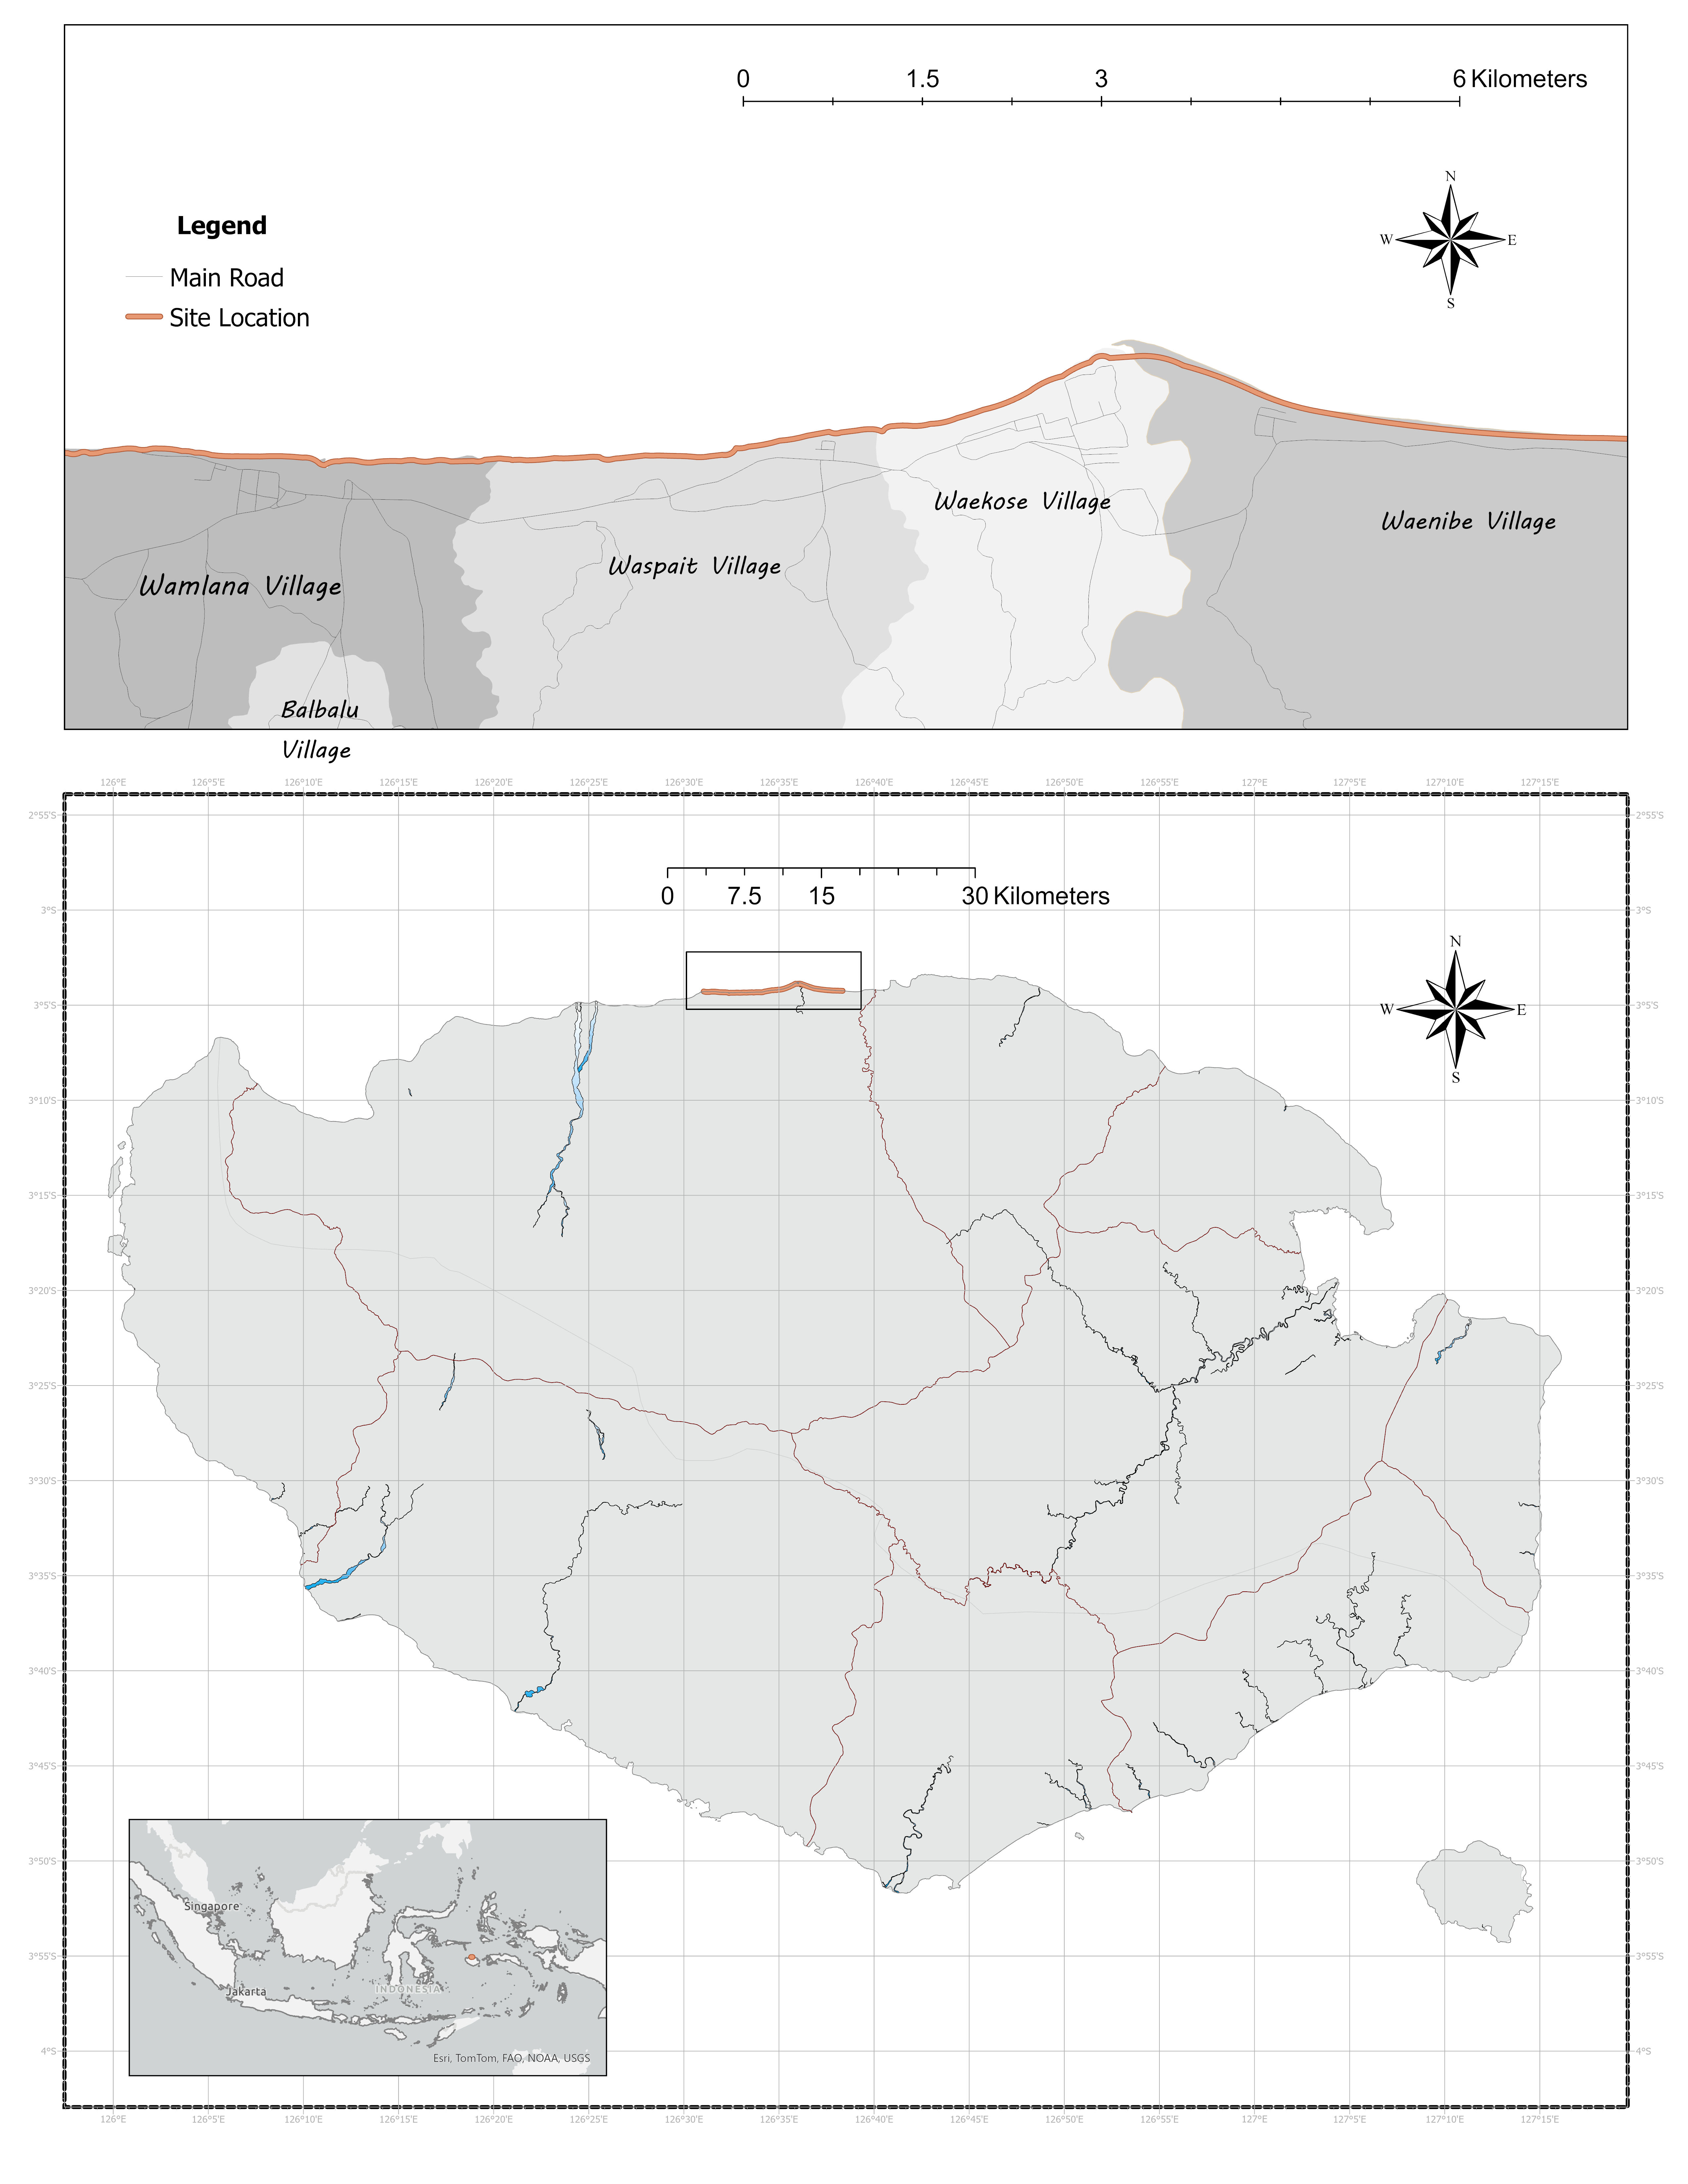
\includegraphics{https://raw.githubusercontent.com/OCN-682-UH/Ningrum/refs/heads/main/week6/week6_homework/data/site_location.jpg}
\caption{\emph{Figure 1. Sea turtle nesting site location, Buru Islan,
Maluku Province, Indonesia}}
\end{figure}

\hypertarget{libraries-needed-for-calculation-and-plot-making}{%
\paragraph{Libraries Needed for calculation and plot
making}\label{libraries-needed-for-calculation-and-plot-making}}

\begin{Shaded}
\begin{Highlighting}[]
\FunctionTok{library}\NormalTok{(ggplot2)         }\CommentTok{\#for data visualization}
\FunctionTok{library}\NormalTok{(dplyr)           }\CommentTok{\#for data manipulation}
\FunctionTok{library}\NormalTok{(here)            }\CommentTok{\#for handling the file path}
\FunctionTok{library}\NormalTok{(tidyverse)       }\CommentTok{\#to tidy the data}
\FunctionTok{library}\NormalTok{(kableExtra)      }\CommentTok{\#to create a table}
\end{Highlighting}
\end{Shaded}

\hypertarget{sea-turtle-nest-distribution-by-villages}{%
\subsection{Sea turtle nest distribution by
villages}\label{sea-turtle-nest-distribution-by-villages}}

\begin{Shaded}
\begin{Highlighting}[]
\NormalTok{df }\OtherTok{\textless{}{-}} \FunctionTok{read\_csv}\NormalTok{(}\FunctionTok{here}\NormalTok{(}\StringTok{"week6"}\NormalTok{, }\StringTok{"week6\_homework"}\NormalTok{, }\StringTok{"data"}\NormalTok{, }\StringTok{"RetnoNingrum\_NestingTurtle\_MBIO612.csv"}\NormalTok{))}

\CommentTok{\#inspect the data}
\CommentTok{\#glimpse(df)}

\CommentTok{\#prepare the data set}
\NormalTok{clean\_df }\OtherTok{\textless{}{-}}\NormalTok{ df }\SpecialCharTok{\%\textgreater{}\%}
  \FunctionTok{filter}\NormalTok{(track\_type }\SpecialCharTok{==} \StringTok{"nesting"}\NormalTok{) }\SpecialCharTok{\%\textgreater{}\%}   \CommentTok{\#use only nesting data}
  \FunctionTok{group\_by}\NormalTok{(beach, species\_id) }\SpecialCharTok{\%\textgreater{}\%}       \CommentTok{\#group by beach name and species name}
  \FunctionTok{summarise}\NormalTok{(}\AttributeTok{total\_nests =} \FunctionTok{n}\NormalTok{()) }\SpecialCharTok{\%\textgreater{}\%}      \CommentTok{\#calculate the amount }
  \FunctionTok{ungroup}\NormalTok{()}

\CommentTok{\#create the plot}
\FunctionTok{ggplot}\NormalTok{(clean\_df,                       }\CommentTok{\#create ggplot use data clean\_df }
       \FunctionTok{aes}\NormalTok{(}\AttributeTok{x =}\NormalTok{ beach,                  }\CommentTok{\#assign x axis with beach name}
           \AttributeTok{y =}\NormalTok{ total\_nests,            }\CommentTok{\#assign y axis with total nest summarised in clean\_df}
           \AttributeTok{fill =}\NormalTok{ species\_id)) }\SpecialCharTok{+}       \CommentTok{\#assign different color to represent each species}
  \FunctionTok{geom\_bar}\NormalTok{(}\AttributeTok{stat =} \StringTok{"identity"}\NormalTok{, }\AttributeTok{position =} \StringTok{"dodge"}\NormalTok{) }\SpecialCharTok{+}   \CommentTok{\#bar plot with bars side by side (dodge) each species}
  \FunctionTok{labs}\NormalTok{(}\AttributeTok{x =} \StringTok{""}\NormalTok{,            }\CommentTok{\#no label in x axis}
       \AttributeTok{y =} \StringTok{"Total Nests"}\NormalTok{, }\CommentTok{\#label in y axis}
       \AttributeTok{caption =} \StringTok{"Figure 2. Sea turtles nest distribution by villages in Buru Island in January 2022 (source : fake data)"}\NormalTok{) }\SpecialCharTok{+}  \CommentTok{\#adding caption}
  \FunctionTok{scale\_fill\_manual}\NormalTok{(}
    \AttributeTok{name =} \StringTok{"Species"}\NormalTok{,    }\CommentTok{\#rename the legend title}
    \AttributeTok{values =} \FunctionTok{c}\NormalTok{(}\StringTok{"gt"} \OtherTok{=} \StringTok{"darkolivegreen"}\NormalTok{, }\StringTok{"or"} \OtherTok{=} \StringTok{"darkgoldenrod4"}\NormalTok{, }\StringTok{"lt"} \OtherTok{=} \StringTok{"dimgrey"}\NormalTok{),  }\CommentTok{\# Specify colors}
    \AttributeTok{labels =} \FunctionTok{c}\NormalTok{(}\StringTok{"gt"} \OtherTok{=} \StringTok{"Chelonia mydas"}\NormalTok{, }\StringTok{"or"} \OtherTok{=} \StringTok{"Lepidochelys olivacea"}\NormalTok{, }\StringTok{"lt"} \OtherTok{=} \StringTok{"Dermochelys coriacea"}\NormalTok{) }\CommentTok{\#rename each labels}
\NormalTok{  ) }\SpecialCharTok{+}
  \FunctionTok{theme\_bw}\NormalTok{() }\SpecialCharTok{+}   \CommentTok{\#using theme\_bw as background template}
  \FunctionTok{theme}\NormalTok{(}
    \AttributeTok{plot.caption =} \FunctionTok{element\_text}\NormalTok{(}\AttributeTok{hjust =} \FloatTok{0.5}\NormalTok{, }\AttributeTok{size =} \DecValTok{14}\NormalTok{),  }\CommentTok{\# Center align caption and set size}
    \AttributeTok{axis.title =} \FunctionTok{element\_text}\NormalTok{(}\AttributeTok{size =} \DecValTok{14}\NormalTok{),   }\CommentTok{\# set axis title size}
    \AttributeTok{axis.text =} \FunctionTok{element\_text}\NormalTok{(}\AttributeTok{size =} \DecValTok{12}\NormalTok{),    }\CommentTok{\# set axis text size}
    \AttributeTok{legend.title =} \FunctionTok{element\_text}\NormalTok{(}\AttributeTok{size =} \DecValTok{14}\NormalTok{), }\CommentTok{\# set legend title size}
    \AttributeTok{legend.text =} \FunctionTok{element\_text}\NormalTok{(}\AttributeTok{size =} \DecValTok{12}\NormalTok{)   }\CommentTok{\# set legend text size}
\NormalTok{  )}
\end{Highlighting}
\end{Shaded}

\begin{center}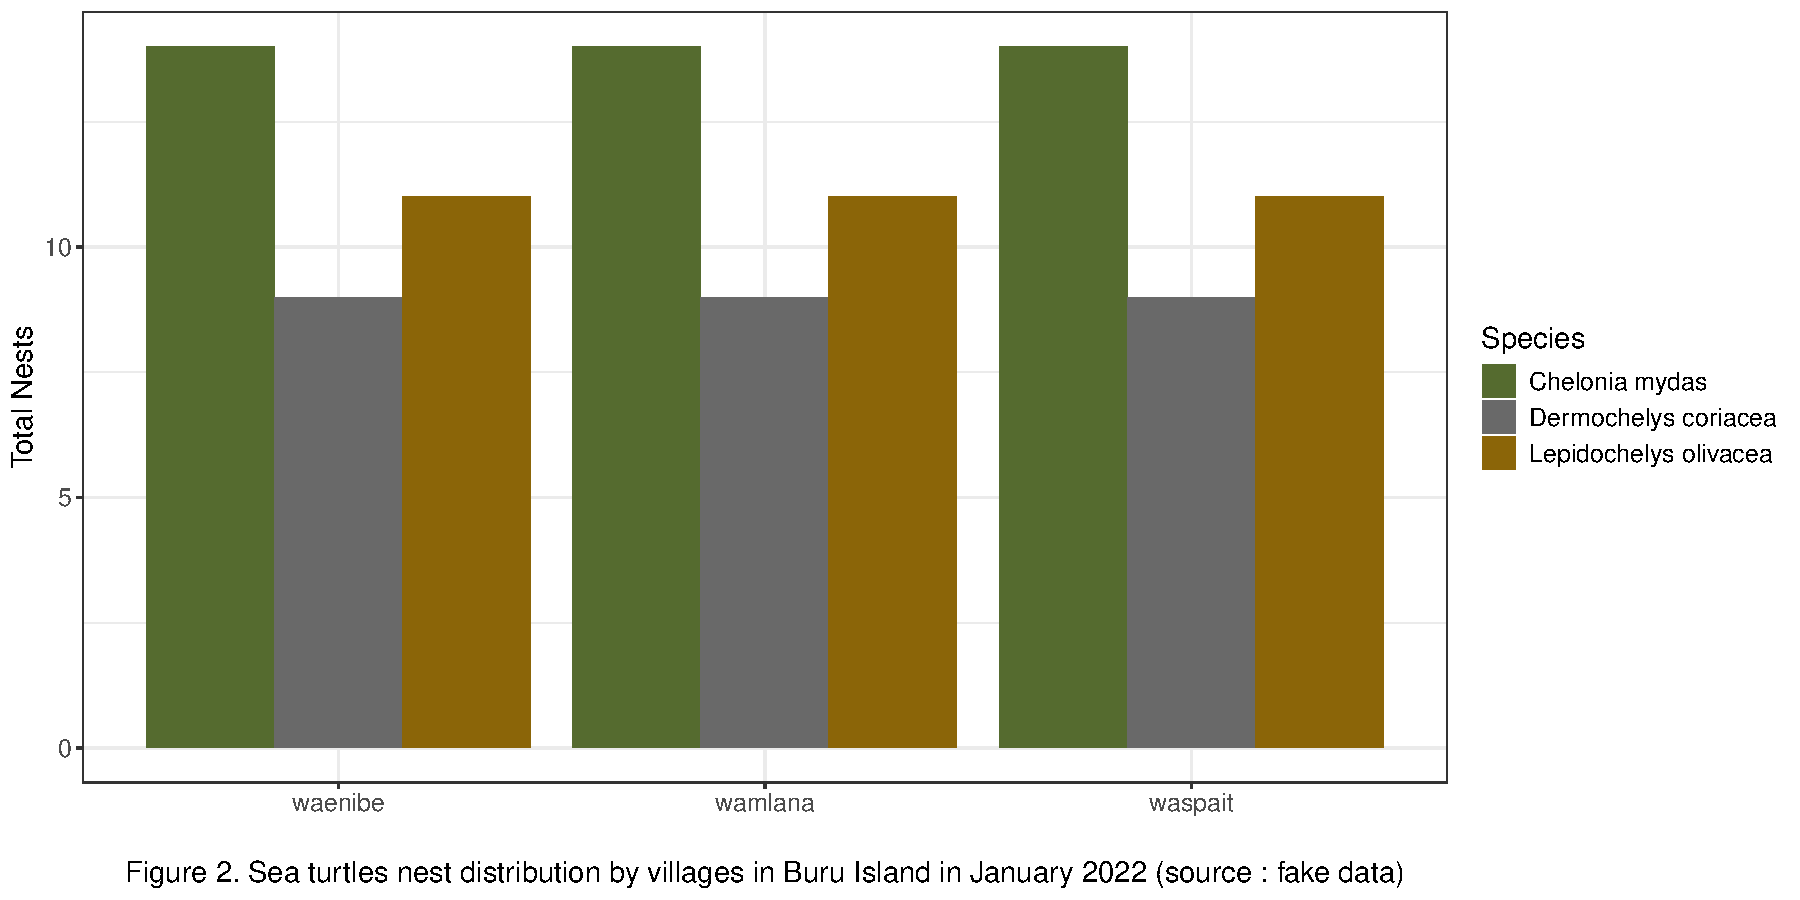
\includegraphics{../output/nest_distribution-1} \end{center}

Overall, the turtles distribution among three villages is similar. The
olive ridley (\emph{Lepodochelys olivacea}) seems to be the majority of
turtles that nest in three beaches. Followed by green turtles
(\emph{Chelonia mydas}) and the least turtle nests found is the
leatherback turtles (\emph{Dermochelys coriacea}). Fun fact about
turtles, turtles often return to the same beach where they were born to
nest. Consequently, with a long-term dataset, we can estimate the
population of female sea turtles in this region.

\hypertarget{sea-turtle-clutch-size}{%
\subsection{Sea Turtle Clutch Size}\label{sea-turtle-clutch-size}}

\begin{Shaded}
\begin{Highlighting}[]
\NormalTok{df }\SpecialCharTok{\%\textgreater{}\%}
  \FunctionTok{filter}\NormalTok{(}\SpecialCharTok{!}\FunctionTok{is.na}\NormalTok{(species\_id)) }\SpecialCharTok{\%\textgreater{}\%}    \CommentTok{\# Remove rows with NA in species\_id}
  \FunctionTok{mutate}\NormalTok{(}\AttributeTok{species =} \FunctionTok{case\_when}\NormalTok{(       }\CommentTok{\# Rename species\_id values}
\NormalTok{    species\_id }\SpecialCharTok{==} \StringTok{"gt"} \SpecialCharTok{\textasciitilde{}} \StringTok{"green turtle"}\NormalTok{,}
\NormalTok{    species\_id }\SpecialCharTok{==} \StringTok{"lt"} \SpecialCharTok{\textasciitilde{}} \StringTok{"leatherback turtle"}\NormalTok{,}
\NormalTok{    species\_id }\SpecialCharTok{==} \StringTok{"or"} \SpecialCharTok{\textasciitilde{}} \StringTok{"olive ridley"}\NormalTok{,}
    \ConstantTok{TRUE} \SpecialCharTok{\textasciitilde{}}\NormalTok{ species\_id               }\CommentTok{\# Keeps the original value if not matched}
\NormalTok{  )) }\SpecialCharTok{\%\textgreater{}\%}
  \FunctionTok{group\_by}\NormalTok{(species, beach) }\SpecialCharTok{\%\textgreater{}\%}                        \CommentTok{\# Group by the new species and beach}
  \FunctionTok{summarise}\NormalTok{(}\AttributeTok{clutch\_size =} \FunctionTok{mean}\NormalTok{(eggs, }\AttributeTok{na.rm =} \ConstantTok{TRUE}\NormalTok{),   }\CommentTok{\# Calculate the mean clutch size}
            \AttributeTok{SE =} \FunctionTok{sd}\NormalTok{(eggs, }\AttributeTok{na.rm =} \ConstantTok{TRUE}\NormalTok{)}\SpecialCharTok{/}\FunctionTok{sqrt}\NormalTok{(}\FunctionTok{n}\NormalTok{()),    }\CommentTok{\# Calculate the SE clutch size}
            \AttributeTok{.groups =} \StringTok{\textquotesingle{}drop\textquotesingle{}}\NormalTok{) }\SpecialCharTok{\%\textgreater{}\%}
  \CommentTok{\# Create the kable table}
  \FunctionTok{kbl}\NormalTok{(}\AttributeTok{caption =} \StringTok{"table.1 sea turtles mean clutch size and standard error by beach "}\NormalTok{) }\SpecialCharTok{\%\textgreater{}\%}
  \FunctionTok{kable\_classic}\NormalTok{() }\SpecialCharTok{\%\textgreater{}\%}                   \CommentTok{\# use the classic theme }
  \FunctionTok{kable\_styling}\NormalTok{(}\AttributeTok{full\_width =} \ConstantTok{FALSE}\NormalTok{)     }\CommentTok{\# FALSE if you want the table not too wide}
\end{Highlighting}
\end{Shaded}

\begin{table}
\centering\centering
\caption{\label{tab:unnamed-chunk-2}table.1 sea turtles mean clutch size and standard error by beach }
\centering
\begin{tabular}[t]{l|l|r|r}
\hline
species & beach & clutch\_size & SE\\
\hline
green turtle & waenibe & 56.6500 & 1.553053\\
\hline
green turtle & wamlana & 56.6500 & 1.553053\\
\hline
green turtle & waspait & 56.6500 & 1.553053\\
\hline
leatherback turtle & waenibe & 78.7500 & 5.225411\\
\hline
leatherback turtle & wamlana & 78.7500 & 5.225411\\
\hline
leatherback turtle & waspait & 78.7500 & 5.225411\\
\hline
olive ridley & waenibe & 57.0625 & 1.911519\\
\hline
olive ridley & wamlana & 57.0625 & 1.911519\\
\hline
olive ridley & waspait & 57.0625 & 1.911519\\
\hline
\end{tabular}
\end{table}

By analyzing the dataset from January 2022, we estimated the clutch size
(total number of eggs in each nest) for each species. Leatherback
turtles exhibited the largest clutch size, averaging 78.7 eggs (SE =
5.2), while green turtles had the smallest average clutch size at 56.6
eggs (SE = 1.5). Olive ridley turtles had a clutch size nearly
equivalent to that of green turtles, with an average of 57 eggs (SE =
1.9) (Table 1).

\hypertarget{sea-turtles-carapace-width-and-carapace-length}{%
\subsection{Sea turtles Carapace width and Carapace
length}\label{sea-turtles-carapace-width-and-carapace-length}}

\begin{Shaded}
\begin{Highlighting}[]
\FunctionTok{ggplot}\NormalTok{(df, }\FunctionTok{aes}\NormalTok{(}\AttributeTok{x =}\NormalTok{ ccl, }\AttributeTok{y =}\NormalTok{ ccw, }\AttributeTok{color =}\NormalTok{ species\_id)) }\SpecialCharTok{+}
  \FunctionTok{geom\_smooth}\NormalTok{(}\AttributeTok{method =} \StringTok{"lm"}\NormalTok{) }\SpecialCharTok{+}
  \FunctionTok{labs}\NormalTok{( }\AttributeTok{x =} \StringTok{"carapace length"}\NormalTok{,}
        \AttributeTok{y =} \StringTok{"carapace width"}\NormalTok{,}
        \AttributeTok{caption =} \StringTok{"Figure 3. The correlation between carapace width and carapace length of sea turtles (source: fake data)"}\NormalTok{) }\SpecialCharTok{+}
  \FunctionTok{scale\_color\_manual}\NormalTok{(}
    \AttributeTok{name =} \StringTok{"Species"}\NormalTok{,}
    \AttributeTok{values =} \FunctionTok{c}\NormalTok{(}\StringTok{"gt"} \OtherTok{=} \StringTok{"darkolivegreen"}\NormalTok{, }\StringTok{"lt"} \OtherTok{=} \StringTok{"dimgrey"}\NormalTok{, }\StringTok{"or"} \OtherTok{=} \StringTok{"darkgoldenrod4"}\NormalTok{),  }\CommentTok{\# Specify colors for each species}
    \AttributeTok{labels =} \FunctionTok{c}\NormalTok{(}\StringTok{"gt"} \OtherTok{=} \StringTok{"Green Turtle"}\NormalTok{, }\StringTok{"lt"} \OtherTok{=} \StringTok{"Leatherback Turtle"}\NormalTok{, }\StringTok{"or"} \OtherTok{=} \StringTok{"Olive Ridley"}\NormalTok{)}
\NormalTok{  ) }\SpecialCharTok{+}
  \FunctionTok{theme\_bw}\NormalTok{() }\SpecialCharTok{+}
  \FunctionTok{theme}\NormalTok{(}
    \AttributeTok{plot.caption =} \FunctionTok{element\_text}\NormalTok{(}\AttributeTok{hjust =} \FloatTok{0.5}\NormalTok{, }\AttributeTok{size =} \DecValTok{14}\NormalTok{),  }\CommentTok{\# Center align caption and increase size}
    \AttributeTok{axis.title =} \FunctionTok{element\_text}\NormalTok{(}\AttributeTok{size =} \DecValTok{14}\NormalTok{),  }\CommentTok{\# Increase axis title size}
    \AttributeTok{axis.text =} \FunctionTok{element\_text}\NormalTok{(}\AttributeTok{size =} \DecValTok{12}\NormalTok{),   }\CommentTok{\# Increase axis text size}
    \AttributeTok{legend.title =} \FunctionTok{element\_text}\NormalTok{(}\AttributeTok{size =} \DecValTok{14}\NormalTok{), }\CommentTok{\# Increase legend title size}
    \AttributeTok{legend.text =} \FunctionTok{element\_text}\NormalTok{(}\AttributeTok{size =} \DecValTok{12}\NormalTok{)   }\CommentTok{\# Increase legend text size}
\NormalTok{)}
\end{Highlighting}
\end{Shaded}

\begin{center}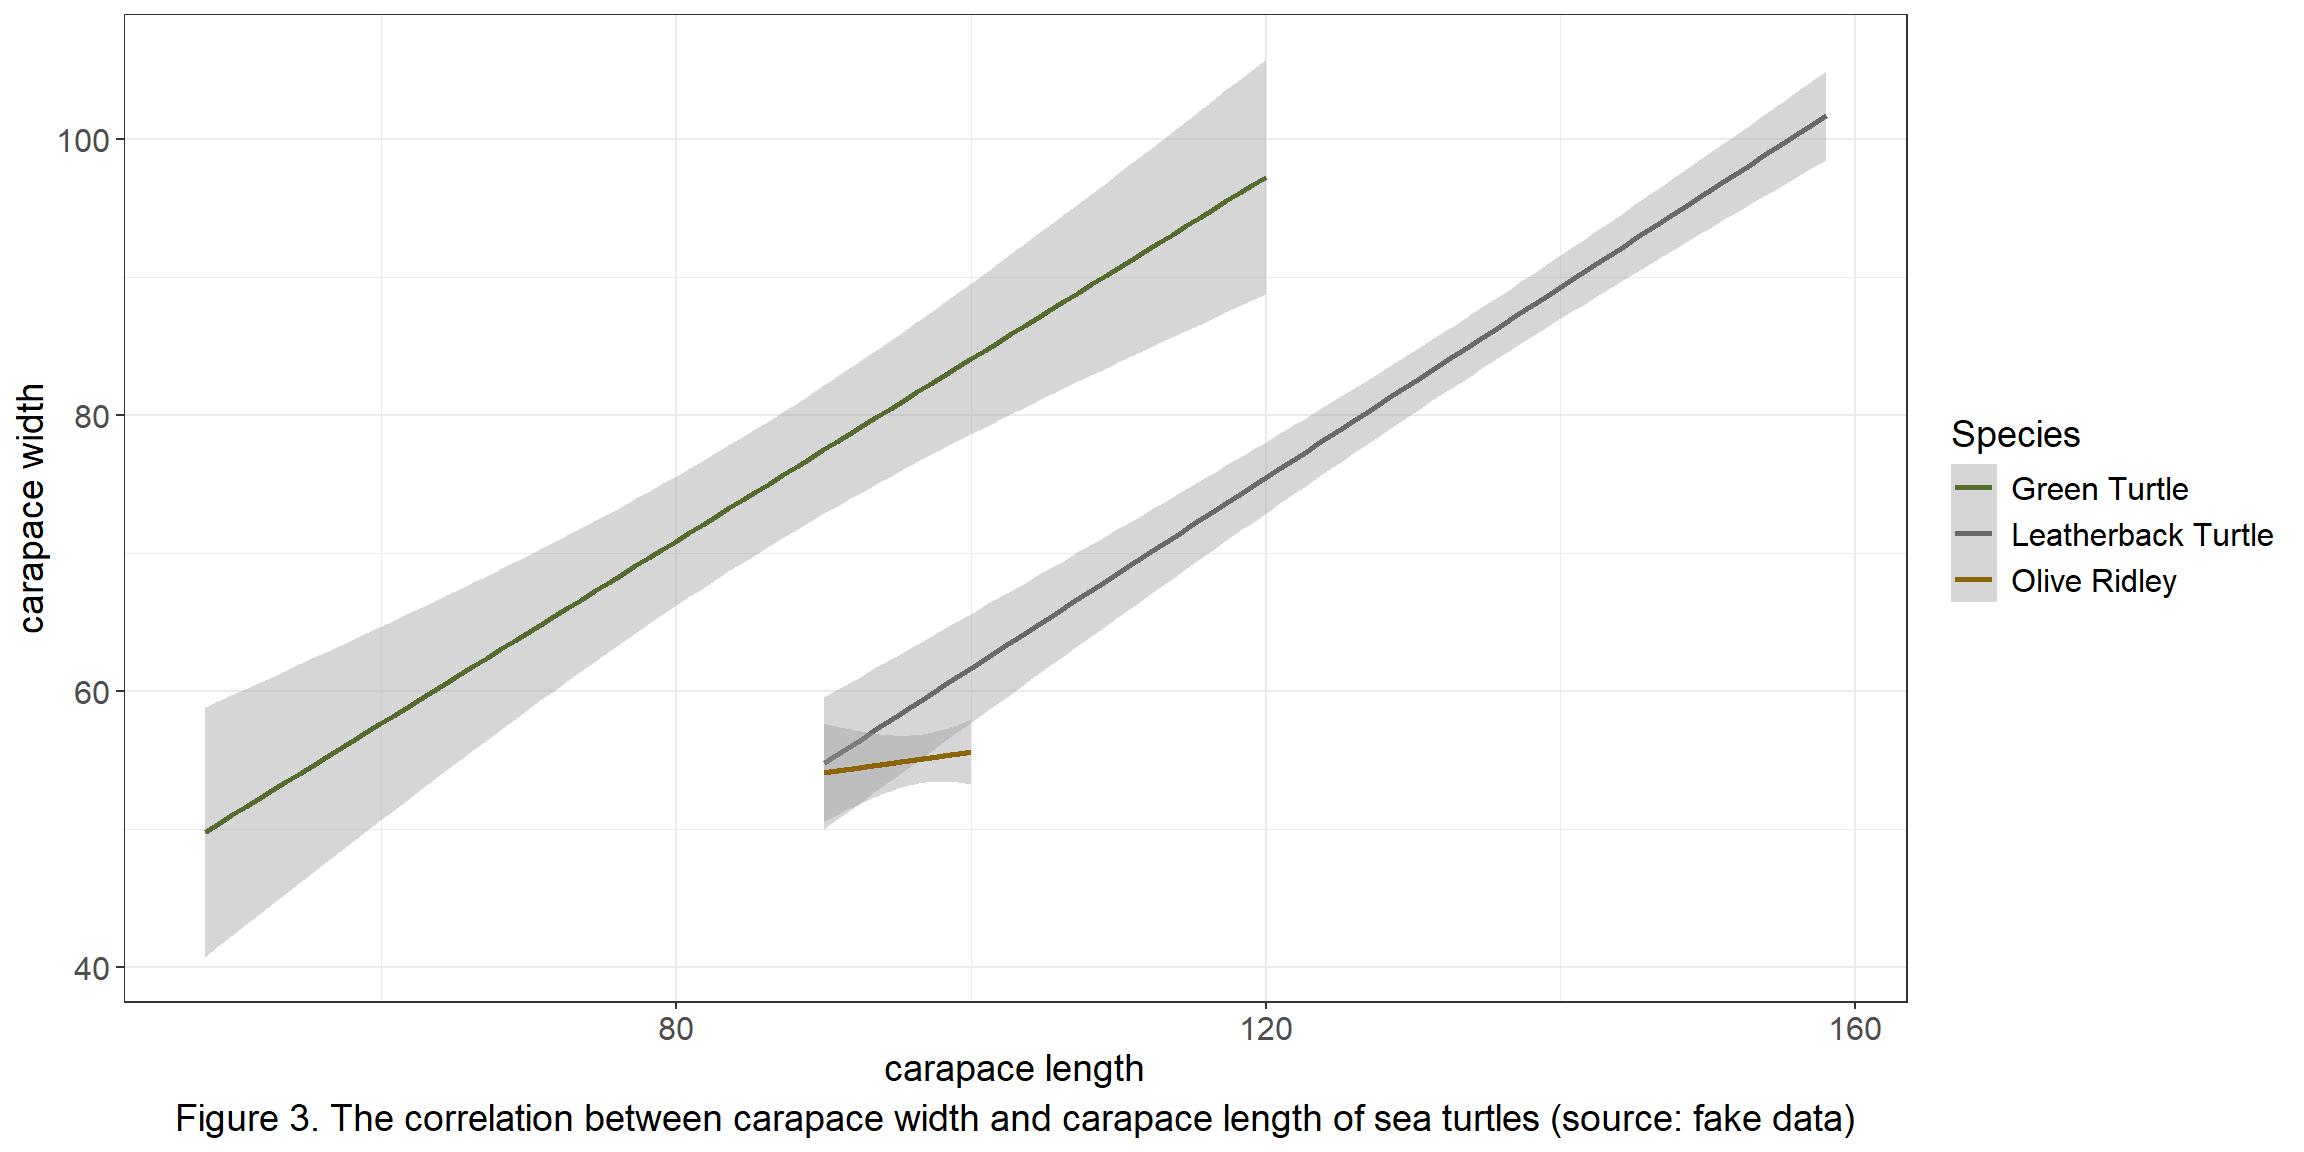
\includegraphics{../output/carapace_correlation-1} \end{center}

Based on the data, all sea turtle species exhibited a similar
correlation, where an increase in carapace length is associated with a
larger carapace width. Overall, leatherback turtles have the largest
carapace size, followed by green turtles, while olive ridley turtles
have the smallest.

\hypertarget{conclusions}{%
\section{Conclusions}\label{conclusions}}

This Rmarkdown document presents an analysis of a \textbf{fake dataset}
about sea turtle nesting sites, focusing on three species: leatherback
turtles (\emph{Dermochelys coriacea}), green turtles (\emph{Chelonia
mydas}), and olive ridley turtles (\emph{Lepidochelys olivacea}). The
findings indicate that olive ridley turtles are the most prevalent
nesters across the studied beaches, followed by green turtles, with
leatherbacks being the least common. The clutch size analysis reveals
that leatherback turtles have the largest average clutch size, while
green turtles exhibit the smallest. Additionally, a correlation analysis
shows that an increase in carapace length corresponds to a larger
carapace width across all species, with leatherback turtles having the
largest dimensions.

\end{document}
